\documentclass[a4paper,12pt]{article} % тип документа

% Поля страниц
\usepackage[left=2.5cm,right=2.5cm,
    top=2cm,bottom=2cm,bindingoffset=0cm]{geometry}
    
%Пакет дял таблиц   
\usepackage{multirow} 
    
%Отступ после заголовка    
\usepackage{indentfirst}


% Рисунки
\usepackage{floatrow,graphicx,calc}
\usepackage{wrapfig}

%%% Работа с картинками
\usepackage{graphicx}  % Для вставки рисунков
\graphicspath{{images/}{images2/}}  % папки с картинками
\setlength\fboxsep{3pt} % Отступ рамки \fbox{} от рисунка
\setlength\fboxrule{1pt} % Толщина линий рамки \fbox{}
\usepackage{wrapfig} % Обтекание рисунков и таблиц текстом

% Создаёем новый разделитель
\DeclareFloatSeparators{mysep}{\hspace{1cm}}

% Ссылки?
\usepackage{hyperref}
\usepackage[rgb]{xcolor}
\hypersetup{				% Гиперссылки
    colorlinks=true,       	% false: ссылки в рамках
	urlcolor=blue          % на URL
}


%  Русский язык
\usepackage[T2A]{fontenc}			% кодировка
\usepackage[utf8]{inputenc}			% кодировка исходного текста
\usepackage[english,russian]{babel}	% локализация и переносы




% Математика
\usepackage{amsmath,amsfonts,amssymb,amsthm,mathtools}

%%% Дополнительная работа с математикой
\usepackage{amsmath,amsfonts,amssymb,amsthm,mathtools} % AMS
\usepackage{icomma} % "Умная" запятая: $0,2$ --- число, $0, 2$ --- перечисление


% Что-то 
\usepackage{wasysym}


\begin{document}
\begin{center}
	\footnotesize{ФЕДЕРАЛЬНОЕ ГОСУДАРСТВЕННОЕ АВТОНОМНОЕ ОБРАЗОВАТЕЛЬНОЕ 			УЧРЕЖДЕНИЕ ВЫСШЕГО ОБРАЗОВАНИЯ}\\
	\footnotesize{МОСКОВСКИЙ ФИЗИКО-ТЕХНИЧЕСКИЙ ИНСТИТУТ\\(НАЦИОНАЛЬНЫЙ 			ИССЛЕДОВАТЕЛЬСКИЙ УНИВЕРСИТЕТ)}\\
	\footnotesize{ФАКУЛЬТЕТ ОБЩЕЙ И ПРИКЛАДНОЙ ФИЗИКИ\\}
	\hfill \break
	\hfill \break
	\hfill \break
	\hfill \break
\end{center}


\begin{figure*}[h]
    \centering
    \includegraphics*[width=10cm,height=7cm,keepaspectratio]{mipt_eng_text_png.png}
    \label{fig:my_label}
\end{figure*}


\begin{center}   
    \hfill \break
	\hfill \break
	\hfill \break
	\large{Лабораторная работа № 4.2.1\\ \hfill \break\Large{Кольца Ньютона}}\\
	\hfill \break
	\hfill \break
	\hfill \break
	\hfill \break
	\begin{flushright}
		Баранов Даниил\\
		Группа Б02-103
	\end{flushright}
	\hfill \break
	\hfill \break
	\hfill \break
\end{center}
\hfill \break
\hfill \break
\hfill \break
\hfill \break
\begin{center}
	Долгопрудный, 2023 г.
\end{center}
\thispagestyle{empty}

\newpage



\textbf{Цель работы}: Познакомиться с явлением интерференции в тонких плёнках (полосы равной толщины) на примере колец Ньютона и с методикой интерференционных измерений кривизны стеклянной поверхности.

\textbf{В работе используются}: Измерительный микроскоп с опак-иллюминатором, плоско-выпуклая линза; пластинка из чёрного стекла, ртутная лампа типа ДРШ, щель, линзы, призма прямого зрения, объектная шкала.

\section{Теоретическая часть}

В нашей установке кольца Ньютона образуются при интерференции световых волн, отражённых от границ тонкой воздушной прослойки, заключённой между выпуклой поверхностью линзы и плоской стеклянной пластинкой.
Линии постоянной разности хода представляют собой концентрические кольца с центром в точке соприкосновения. Радиусы тёмных и светлых колец определяются формулами \eqref{dark} и \eqref{light} соответственно. Для протяжённого источника линии равной толщины локализованы на поверхности линзы, если пластинка лежит на линзе, и вблизи поверхности линзы, если линза лежит на пластинке, как в нашем случае. Наблюдение ведётся в отражённом свете.

\begin{equation}
    r_m = \sqrt{m\lambda R}
    \label{dark}
\end{equation}

\begin{equation}
    r_m' = \sqrt{(2m-1)m\lambda R/2}
    \label{light}
\end{equation}

\section{Экпериментальная установка}

Схема экспериментальной установки приведена на рис. \ref{ust}. Опыт выполняется с помощью измерительного микроскопа. На столике микроскопа помещается держатель с пластинкой чёрного стекла. На пластинке лежит исследуемая линза.
Источником света служит ртутная лампа, находящаяся в защитном кожухе. Для получения монохроматического света применяется призменный монохроматор, состоящий из конденсора $K$, коллиматора (щель $S$ и объектив $O$) и призмы прямого зрения $\Pi$. Эти устройства с помощью рейтеров располагаются на оптической скамье. Свет от монохроматора попадает на опак-иллюминатор (ОИ), расположенный между окуляром и объективом микроскопа -- специальное устройство для освещения объекта при работе в отражённом свете. Внутри опак-иллюминатора находится полупрозрачная пластинка $P$, наклоненная под углом 45$^\circ$ к оптической оси микроскопа. Свет частично отражается от этой пластинки, проходит через объектив микроскопа и попадает на исследуемый объект. Пластинка может поворачиваться вокруг горизонтальной оси $x$, а опак-иллюминатор -- вокруг вертикальной оси.

\begin{figure}[H]
    \centering
    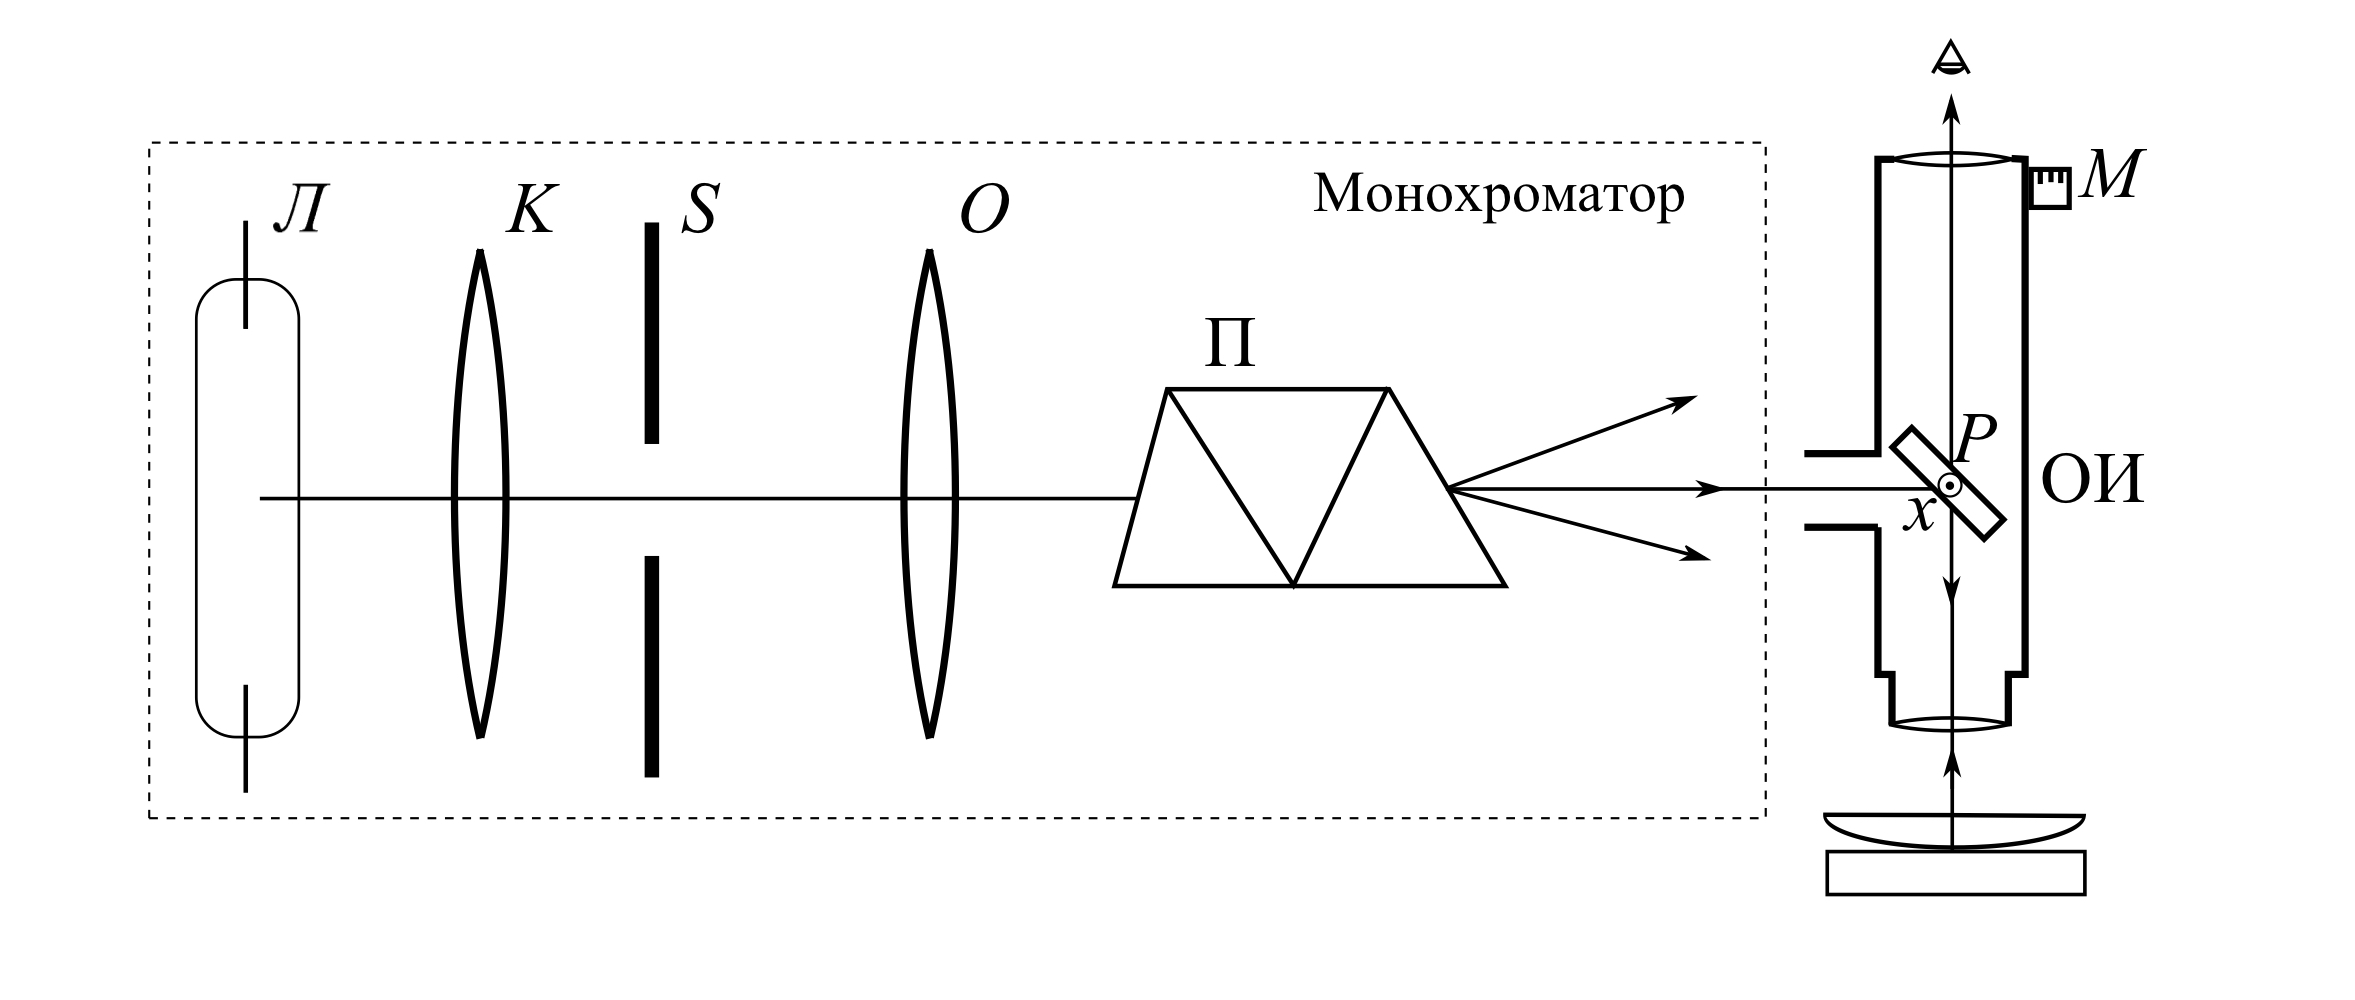
\includegraphics[scale=0.2]{4.2.1/ustan.jpeg}
    \caption{Схема установки для наблюдения колец Ньютона}
    \label{ust}
\end{figure}

Столик микроскопа может перемещаться в двух взаимно перпендикулярных направлениях с помощью винтов препаратоводителя. Отсчетный крест окулярной шкалы перемещается перпендикулярно оптической оси микроскопа с помощью микрометрического винта.
Оптическая схема монохроматора позволяет получить в плоскости входного окна опак-иллюминатора достаточно хорошо разделённые линии спектра ртутной лампы. Изображение щели $S$ фокусируется на поверхность линзы объективом микроскопа, и в том же месте находится плоскость наблюдения микроскопа, т.е. точка источника и точка наблюдения интерференции совпадают. Картина интерференции как и в случае расположения пластинки сверху, так и в данном случае не зависит от коэффициента преломления линзы и определяется величиной зазора между нижней поверхностью линзы и стеклянной пластинкой.
Рекомендуется сначала настроить микроскоп на кольца Ньютона в белом свете (свете ртутной лампы), а затем после выделения монохроматором зелёной линии провести измерения в монохроматическом свете.

\section{Ход работы и полученные данные}

\subsection{Определение радиуса кривизны линзы}

Для определения радиуса кривизны линзы измеряют диаметры колец: устанавливают перекрестие на середину какого-либо достаточно удалённого от центра, но ещё отчётливо видимого тёмного кольца и снимают отсчёт по окулярной шкале: целые деления отсчитываются слева от риски, проходящей через окулярную шкалу, десятые и сотые доли деления — по окулярному микрометрическому винту $M$.
Перемещая перекрестие, последовательно устанавливают его на середины тёмных колец и записывают соответствующие показания окулярной шкалы и микрометра. После прохождения через центральное пятно продолжают измерения, записывая возрастающие номера колец и координаты их диаметров. Для устранения ошибок, возникающих из-за люфта в винте, перекрестие всегда следует подводить к кольцу с одной стороны. Цену одного деления окулярной шкалы определяют сравнивая её с изображением эталонной (объектной) шкалы. По разности отсчётов определяют диаметры, а затем и радиусы тёмных колец. Аналогичная серия измерений выполняется для светлых колец Ньютона.

Полученные данные приведены в таблице \ref{radi}

\begin{table}[H]
    \centering
    \begin{tabular}{|c|c|c|c|c|}
        \hline $m$ & $D_m$, дел & $D_m'$, дел & $\varepsilon_D$, \% & $\varepsilon_D'$, \% \\ \hline
        1 & 1,79 & 1,27 & 5,6 & 7,9 \\ \hline
        2 & 2,48 & 2,08 & 4,0 & 4,8 \\ \hline
        3 & 3,09 & 2,80 & 3,2 & 3,6 \\ \hline
        4 & 3,50 & 3,28 & 2,9 & 3,0 \\ \hline
        5 & 3,93 & 3,71 & 2,5 & 2,7 \\ \hline
        6 & 4,28 & 4,10 & 2,3 & 2,4 \\ \hline
        7 & 4,62 & 4,46 & 2,2 & 2,2 \\ \hline
    \end{tabular}
    \caption{Диаметры тёмных и светлых колец}
    \label{radi}
\end{table}

\subsection{Наблюдение ''Биений''}

При освещении системы светом, содержащим две спектральные компоненты, наблюдается характерная картина биений: чёткость интерференционных колец периодически изменяется. Это объясняется наложением двух систем интерференционных колец, возникающих для разных длин волн $\lambda_1$ и $\lambda_2$. Чёткие кольца в результирующей картине образуются при наложении светлых колец на светлые и тёмных на тёмные. Размытые кольца получаются при наложении светлых колец одной картины на тёмные кольца другой.
Нетрудно рассчитать период возникающих биений. Пусть в промежутке между двумя центрами соседних чётких участков укладывается $\Delta m$ колец для спектральной линии с длиной волны $\lambda_1$. Тогда в этом промежутке должно располагаться $(\Delta m + 1)$ колец для спектральной линии с длиной волны $\lambda_2$ (при $\lambda_2$ < $\lambda_1$).
Получаем соотношение \eqref{m}.

\begin{equation}
    \Delta \lambda = \lambda_2 / m
    \label{m}
\end{equation}

В процессе выполнения работы было получено $\Delta m = 14$. Из этого следует, что $\displaystyle \Delta \lambda \approx 39 \ (\lambda_2 = 546 \text{нм})$. Этот результат отличается от табличного на 6 нм (в большую сторону).

\subsection{Калибровка окулярной шкалы}

Для определения цены деления окулярной шкалы сверху на линзу кладут калиброванную объектную шкалу. Плавно поднимая тубус, находят изображение миллиметровой шкалы и совмещают его с окулярной шкалой.
Объектная шкала размером 1 мм разбита на 100 делений. Используя всё поле зрения микроскопа, отмечают, какие из самых дальних штрихов объектной шкалы лучше всего совпадают со штрихами окулярной шкалы. Можно использовать для калибровки окулярный микрометр, совмещая перекрестие с началом и концом объектной шкалы.

Оказалось, что одно деление окулярной шкалы с высокой точностью соответствует 0,1 мм.

\section{Обработка результатов}

По данным таблицы \ref{radi} был построен график на рис. \ref{graph}. 

\begin{figure}[H]
    \centering
    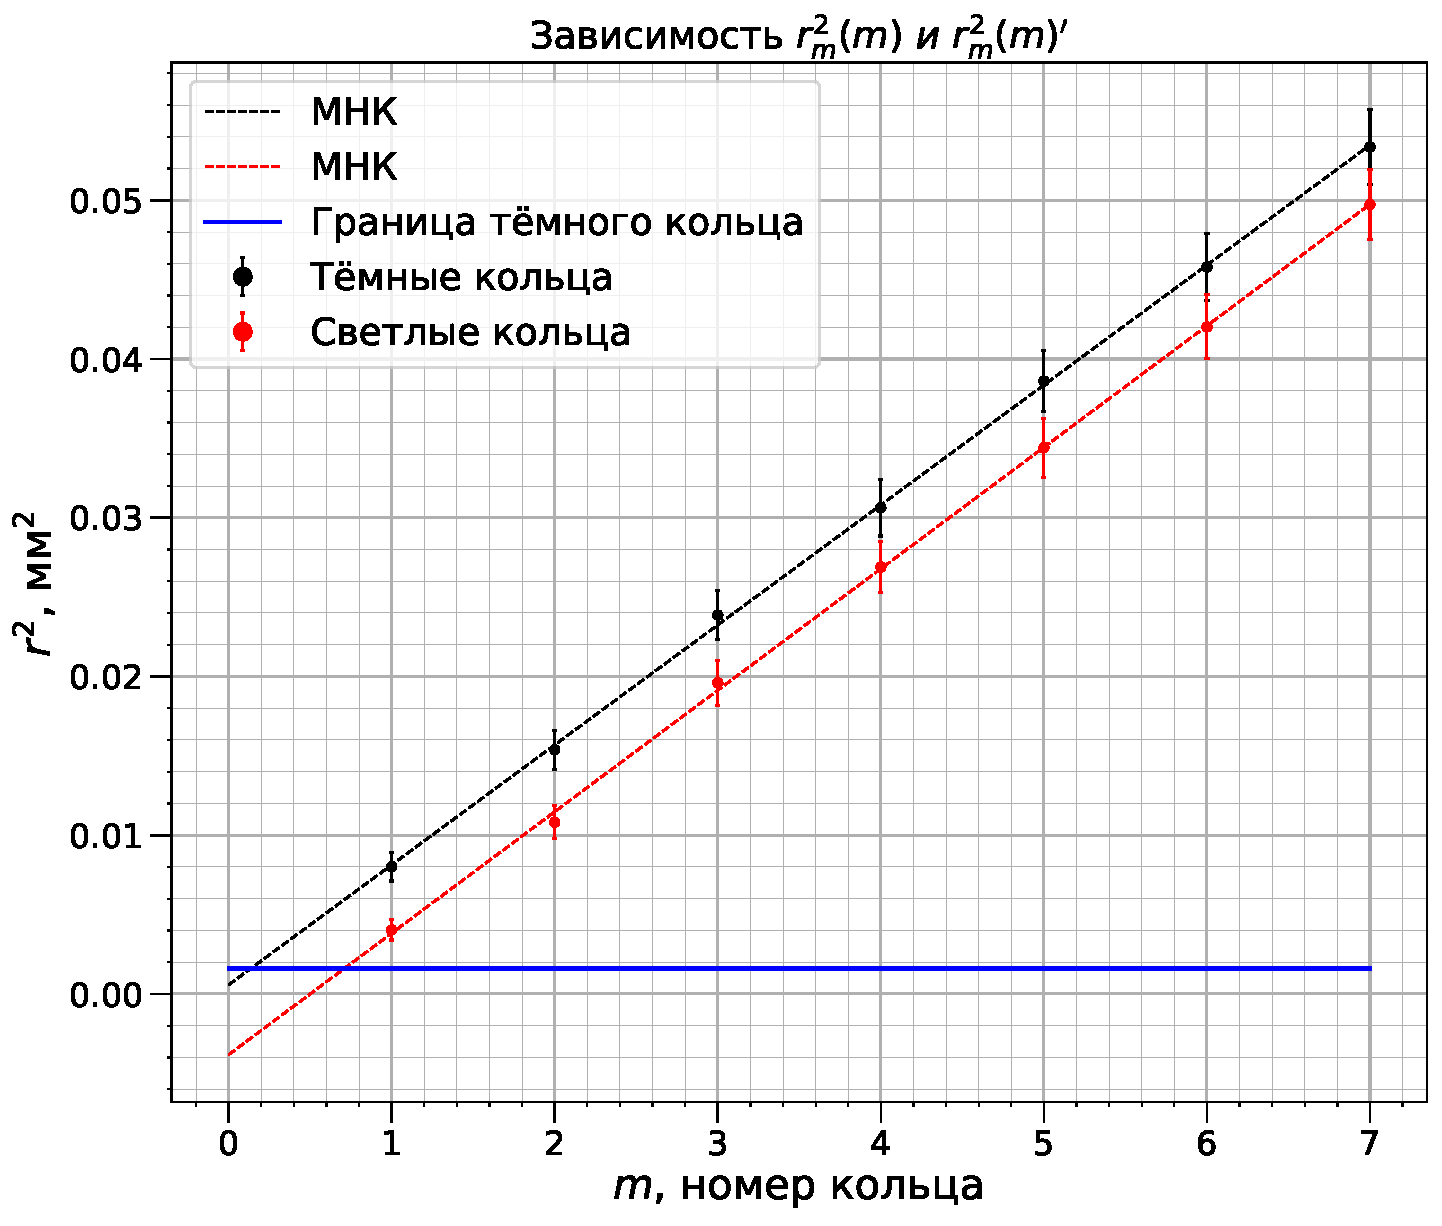
\includegraphics[scale=0.65]{r2(m).pdf}
    \caption{График зависимости $r_m^2$ и $r_m^2'$}
    \label{graph}
\end{figure}

Угол наклона соствил $k =7,67 \pm 0,06 \cdot 10^{-3}$ мм$^2$ (из МНК). Можем найти радиус линзы из формулы:

\begin{equation}
    R = \frac{k}{\lambda_2}
\end{equation}

Окончательно, получаем $R = 14,0 \pm 0,1$ мм.

\section{Выводы}

Таким образом, мы получили, что их экспериментального периода биений разница длин волн  желтого и зеленого света ртутной лампы примерно равна $  \Delta \lambda = 39 \text{ нм} $, в то время как табличный результат --- 33 нм. Отклонение может быть объяснено неточностью k в связи со сложностью подсчета в зоне малой видности $ \Delta m $.
	
Также мы построили графики зависимости радиусов колец Ньютона от их номеров. Полученный результат позволил нам рассчитать радиус линзы ---  $ R = 1,40 \pm 0,01 \text{ см} $.


\end{document}
